\documentclass[11pt, a4paper, titlepage, oneside]{scrbook}

\usepackage{../Tarc/Tarc}
\usepackage{../Tarc/Tarc-private}
\graphicspath{{immagini/}}

\title{Basi di Dati}
\author{Lorenzo Ferraro}
\date{\today}
\setDegree{Informatica}

\begin{document}

\frontmatter
\SapienzaCoverItalianoTriennale
\InfoSegnalazioni

\tableofcontents

\mainmatter

\chapter{Introduzione alle basi di dati}

\section{Sistema informativo}

\begin{Definizione}[Sistema informativo]
\label{def-sistema-informativo}
Un \textbf{sistema informativo} di un'organizzazione è una combinazione di risorse, umane e materiali, e di procedure organizzate per \textit{raccogliere}, \textit{archiviare}, \textit{elaborare} e \textit{scambiare} le informazioni necessarie alle attività \textbf{operative} (informazioni di serivizio), di \textbf{programmazione e controllo} (informazioni di gestione) e di \textbf{pianificazione strategica} (informazioni di governo).
\end{Definizione}

Questo sistema è quindi una componente dell'organizzazione che viene utilizzata per gestire le infromazioni di interesse, supportando  le altre componenti dell'organizzazione (come il sistema produttivo o decisionale, ad esempio). 

\begin{Definizione}[Sistema informatico]
\label{def-sistema-informatico}
Il \textbf{sistema informatico} è l'insieme delle tecnologie informaitche e della comunicazione (ICT) a supporto delle attività di un'organizzazione.
\end{Definizione}

\begin{Definizione}[Sistema informativo automatizzato]
\label{def-sistema-informativo-automatizzato}
Il \textbf{sistema informativo automatizzato} è quella parte del sistema informativo dove le informazioni sono raccolte, elaborate, archiviate e scambiate tramite l'ausilio di un sistema informatico.
\end{Definizione}

Dato che ormai quasi tutti i sistemi informativi sono digitalizzati, i tre termini appena visti tendono spesso a sovrapporsi e a essere usati come sinomini.

\section{Gestione dei dati}

Negli anni 60'/70' ogni applicazione aveva un proprio file privato dove venivano salvati i propri dati. Questo creava una serie di problemi:
\begin{itemize}
    \item \textbf{ridondanza}, dato che se due applicazioni usavano gli stessi dati questi venivano salvati due volte.
    \item \textbf{inconsistenza}, dato che aggiornare un dato in un file non significava aggiornarlo automaticamente in tutti i file
    \item \textbf{dipendenza dei dati}, dato che ogni applicazione organizzava i propri dati tenendo conto solamente dell'uso che doveva farne
\end{itemize}

Proprio per questo motivo nascono le \textbf{basi di dati}.

\begin{Definizione}[Basi di Dati]
\label{def-basi-di-dati}
Una \textbf{Base di Dati} (o Database, \textbf{DB}) è un \textbf{insieme di file connessi tra loro}. Gli insiemi di dati sono organizzati in delle \textit{strutture di dati} che rendono più facile la creazione, l'accesso e l'aggiornamento di tali e ottimizzano la gestione delle risorse fisiche.
\end{Definizione}

\begin{Definizione}[Dati]
\label{def-dati}
I \textbf{dati} sono dei fatti grezzi che bisogna interpretare e correlare per fornire una vera informazione.
\end{Definizione}

Ad esempio, 3336669990 da solo è un semplice numero, ma se è la risposta alla domanda "Qual è il numero di telefono di X", allora ha tutto un altro significato, e diventa quindi una \textit{informazione} vera e propria.

Quando si registrano delle informazioni, questi possono essere
\begin{itemize}
    \item \textbf{dati strutturati}, ossia rappresentati da brevi stringhe di simboli e da numeri,
    \item o \textbf{dati non strutturati}, ossia testi scritti in linguaggio naturale.
\end{itemize}

La struttura dell'informazione dipende dal suo utilizzo e può essere modificata. Ad esempio, un tempo bastava il nome e il cognome di una persona per identificarla in modo efficace, mentre oggi utilizziamo anche la data di nascita, il luogo di nascita e, se necessario, il codice fiscale. 

L'obiettivo di una base di dati non è solo il memorizzare i dati in modo compatto, ma soprattutto \textbf{facilitarne l'elaborazione} sulla base delle loro relazioni. Ad esempio, parlando dei dati strutturati, vi si può accedere singolarmente tramite delle "interrogazioni", dette \textit{query}, e le relazioni tra i dati individuali sono salvate nella \textit{struttura dei record}. 

I dati contenuti DB sono suddivisi in due categorie:
\begin{itemize}
    \item \textbf{dati}: rappresentazioni di fatti conformi alla definizione dello scheam delle basi di dati. Questi hanno diverse caratteristiche:
    \begin{itemize}
        \item Sono organizzati in insieme strutturati e omogenei, con relazioni definite tra i vari insiemi.
        \item Sono molti di più rispetto ai metadati, e non sono gestiti nella RAM (memoria temporanea).
        \item Sono accessibili tramite transazioni, sequenze di istruzioni che devono tutte andare a buon fine per apportare vere modifiche.
        \item Sono protetti sia dall'accesso di utenti non autorizzati, sia da malfunzionamento di hardware e/o software.
        \item Sono utilizzabili contemporaneamente da più utenti.
    \end{itemize}
    \item \textbf{metadati}: descrivono fatti sullo schema dei dati, utenti autorizzati, applicazioni e così via. Sono descritti da uno schema e sono interrogabili come i dati.
\end{itemize}

\begin{Definizione}[Sistemi di Gestione di Basi di Dati]
\label{def-sistemi-gestione-basi-dati}
I \textbf{Sistemi di Gestione di Basi di Dati} (o Database Management System, \textbf{DBMS}) sono \textbf{software per la gestione di molti dati} che si trovano nella memoria secondaria.
\end{Definizione}

Questi offrono gli strumenti per \textbf{definire lo schema} di un DB, che va definito prima di inserire i dati, per \textbf{scegliere le strutture dati adeguate}, per \textbf{memorizzare i dati} rispettando i vincoli dello schema scelto, e per \textbf{recuperare/modificare} i dati in modo interattivo o attraverso dei programmi. Sono dunque il ponte tra gli utenti e il DB vero e proprio.

\subsection{Informazioni condivise}

In un'organizzazione, ogni componente è interessata a una porzione del Sistema Informativo. Quando queste porzioni si sovrappongono, la base di dati diventa fondamentale, facendo da \textit{struttura condivisa} tra tutte le componenti, riducendo le ridondanze e le inconsistenze. Questa condivisione, però, non è sempre completa. Infatti, non tutte le componenti dell'organizzazione possono accedere a tutti i dati di questa: le informazioni più private devono essere salvaguardate. Inoltre, la condivisione comporta la necessità di gestire accessi in contemporanea sugli stessi dati: questo è il problema del \textbf{controllo della concorrenza}. 

\section{Sistemi informatici}

I sistemi informatici si dividono in due macrogruppi:
\begin{itemize}
    \item \textbf{sistemi informatici operativi}
    \item \textbf{sistemi informatici di supporto alle decisioni} (direzionali)
\end{itemize}

\subsection{Sistemi informatici operativi}

I \textbf{sistemi informatici operativi} (o Data processing, DP / Electronic Data processing, EDP / Transaction Processing Systems, TPS) sono organizzati in basi di dati. Qui le applicazioni sono usate per svolgere le attività strutturate e ripetitive di un'azienda nell'area amministrativa e finanziaria. Abbiamo quindi una base di dati, gestita da un DBMS, che lavora con più applicazioni in ambiti come la vendita, la contabilità, la finanza...

\begin{Definizione}[OLTP]
\label{def-OLTP}
L'\textbf{OLTP} (On-Line Transaction Processing) è il \textbf{paradigma architetturale} usato dai DBMS nei sistemi informatici operativi. Le sue operazioni sono predefinite e relativamente semplici, e ognuna di queste coinvolge pochi dati, che sono però dettagliati e aggiornati.
\end{Definizione}

\subsection{Sistemi informatici di supporto alle decisioni}

I dati nei \textbf{sistemi informatici di supporto alle decisioni} (Decision Support Systems, DSS / Management Information Systems, MIS / Executive Information System, EIS) sono organizzati in \textbf{Data Warehouse} (DW) e gestiti da un sistema apposito. Le applicazioni, dette di \textit{Business Intelligence}, supportano i processi di controllo delle prestazioni aziendali e di decisione manageriale. Abbiamo quindi una base di dati operazionale e dei possibili dati esterni che vanno dentro il DW che viene gestito da un DBMS dedicato, e infine il sistema OLAP (che ora vedremo) interroga il DW e fornisce le informazioni necessarie agli strumenti di Business Intelligence.

\begin{Definizione}[OLAP]
\label{def-OLAP}
L'\textbf{OLAP} (On-Line Analytical Processing) è il \textbf{paradigma} usato nei DSS per analizzare i dati. Le sue operazioni sono complesse e casuali, e ognuna coinvolge molti dati, che sono aggregati, storici e non sempre molto attuali.  
\end{Definizione}

\subsection{OLTP vs OLAP}

Vediamo le molte differenze tra OLTP e OLAP.
\begin{itemize}
    \item L'OLTP supporta \textbf{l'operatiivà} dell'azienda, mentre l'OLAP le sue \textbf{decisioni}
    \item L'OLTP ha \textbf{molti utenti}, mentre l'OLAP è più \textbf{esclusivo}
    \item I dati dell'OLTP sono \textbf{analitici e relazionali}, mentre quelli dell'OLAP sono \textbf{sintetici} e \textbf{multidirezionali}
    \item Gli utilizzi dell'OLTP sono \textbf{noti a priori}, mentre quelli dell'OLAP \textbf{non sono molto prevedibili}.
    \item Per attività, la quantità di dati dell'OLPT è \textbf{bassa} (si parla di decine di dati), mentre quella dell'OLAP è \textbf{alta} (si parla di milioni di dati)
    \item L'OLTP è \textbf{orientato all'applicazione}, mentre l'OLAP al \textbf{soggetto}
    \item Nell'OLTP gli aggiornamenti sono \textbf{frequenti}, mentre nell'OLAP sono \textbf{rari}
    \item Nell'OLTP i dati sono \textbf{sovrascritti} (i dati vecchi non sono interessanti), mentre nell'OLAP sono \textbf{importanti anche i dati vecchi}
    \item L'OLTP è ottimizzato per le \textbf{transazioni}, mentre l'OLAP per l'\textbf{analisi dei dati}
\end{itemize}

\subsection{Requisiti per l'analisi dei dati}

I dati dell'OLAP sono presi per essere analizzati. Questi hanno bisogno di requisiti specifici:
\begin{itemize}
    \item Devono essere \textbf{aggregati}: non ci interessa il singolo dato, ma un calcolo su più dati, come la somma, la media o la mediana.
    \item Le informazioni devono essere \textbf{incrociate}: bisogna spesso analizzare i dati da punti di vista diversi.
    \item Bisogna analizzare i dati su \textbf{diversi livelli di dettaglio}: ad esempio, se si scopre un calo nelle vendite in un periodo di una regione, bisogna analizzare quei dati in modo più approfondito per capirne le cause 
\end{itemize}

I sistemi informatici operativi, essendo progettati per un'elaborazione rapida delle transazioni, sono dunque l'\textbf{perfetti per OLTP} ma non adatti per l'OLAP.

\section{Big Data e Data Lake}

\begin{Definizione}[Big Data]
\label{def-big-data}
\textbf{Big Data} è un termine ampio che si riferisce a tutte le situazioni dove l'approccio \textit{schema-first} tipico dei DB e delle DW è troppo lento o restrittivo. Si parla in questo caso delle 3 V:
\begin{itemize}
    \item \textbf{Volume}
    \item \textbf{Varietà}
    \item \textbf{Velocità}
\end{itemize}
Sono questi 3 fattori a mandare in crisi i sistemi tradizionali (quantità di dati o eccessive, o troppo variegate, o dati che devono essere elaborati velocemente).
\end{Definizione}

I Big Data sono associati solitamente ai sistemi NoSQL, al Machine Learning, e all'\textbf{approccio Data Lake}.

\begin{Definizione}[Data Lake]
\label{def-data-lake}
Un \textbf{Data Lake} è un \textbf{ambiente di data storage} a basso costo creato per gestire enormi quantità di dati non elaborati e di qualsiasi formati, inclusi dati strutturati, semi-strutturati e non strutturati.
\end{Definizione}

Quasi tutti i Data Lake utilizzano lo storage a ogetti basato su cloud, come Google Cloud Storage. Questi sono nati per gestire il flusso di nuovi big data, molti non strutturati, creati da app e servizi conessi a Internet. A differenza dei DB e DW tradizionali, questi non richiedono uno schema di dati definito e possono anche memorizzare diversi tipi di dati in più formati tutti nello stesso posto. Questo li rende più ideali per i data scientist, grazie al suo schema \textit{on-read}: i dati vengono strutturati solo quando vanno letti, al contrario dello schema \textit{on-write} delle DW dove i dati sono strutturati fin da subito.

\section{Modelli di DBMS}

\subsection{Prima del modello relazionale}

Il modello relazionale è ad oggi lo standard per i DBMS. Lo analizzeremo tra poco, ma per ora diamo un occhiata ai modelli che lo hanno preceduto.

Il primo modello di DB è il \textbf{modello gerarchico}, uscito a metà degli anni 60'. Questo organizza i dati in una struttura ad albero dove ogni record figlio può avere solo un genitore. Questo modello è stato poi esteso dal modello \textbf{reticolare}, che ha trasformato l'albero (che è un grafo acircolare e connesso) in un grafo generico.

A metà degli anni 80' arrivano anche i primi sistemi \textbf{orientati a oggetti}. In questo modello troviamo gli \textit{attributi} che descrivono lo stato di un oggetto, e i \textit{metodi} che ne descrivono invece il comportamento. Al contrario del modello relazionale, però, non esisteancora un modello universalmente riconosciuto.

\subsection{Modello relazionale}

\begin{Definizione}[Modello relazionale]
\label{def-modello-relazionale}
Nel 1970 E.F. Codd, lavorando per IBM, idea il \textbf{modello relazionale}, che diventerà lo standard nel 1993. Qui \textbf{dati e relazioni sono rappresentati entrambi come valori}. Non ci sono puntatori espliciti come nei modelli reticolari e gerarchici, portando l'astrazione ad un livello più in alto.
\end{Definizione}

I record sono gli \textbf{oggetti}, mentre le informazioni di interesse sono i \textbf{campi}. Lavoriamo con delle \textbf{tabelle} di oggetti omogenei, dove le colonne sono rappresentate dai campi mentre le righe dagli oggetti appunto. Vediamo un esempio di DB relazionale:

\newpage

\begin{table}[!t]
  \centering
  \begin{minipage}[t]{0.48\textwidth}
    \centering
      \caption*{Studenti}
    \small
    \begin{tabular}{|c|c|c|c|}
      \hline
      \textbf{Matricola} & \textbf{Nome} & \textbf{Cognome} \\
      \hline
      123456 & Mario & Rossi  \\
      654321 & Andrea & Pirlo  \\
      456789 & Francesco & Totti \\
      987654 & Cristiano & Ronaldo \\
      \hline
    \end{tabular}
  \end{minipage}\hfill
  \begin{minipage}[t]{0.48\textwidth}
    \centering
    \small
      \caption*{Corsi}
    \begin{tabular}{|c|c|c|}
      \hline
      \textbf{Codice} & \textbf{Titolo} & \textbf{Insegnante} \\
      \hline
      01 & Analisi & Aiello \\
      02 & Chimica & Sterbini \\
      03 & Fisica & Carlucci \\
      \hline
    \end{tabular}
  \end{minipage}
\end{table}

\begin{table}[!t]
    \centering
    \small
      \caption*{Esami}
    \begin{tabular}{|c|c|c|}
      \hline
      \textbf{Studente} & \textbf{Voto} & \textbf{Corso} \\
      \hline
      123456 & 21 & 02 \\
      987654 & 30 & 03 \\
      456789 & 28 & 01 \\
      \hline
    \end{tabular}
\end{table}

Notiamo come le relazioni tra i diversi oggetti siano rappresentate dai valori stessi appunto: nella tabella Esami, riusciamo a capire chi ha svolto quale esame e ha preso quale voto grazie ai valori nella tabella. Ad esempio, capiamo che Mario Rossi ha preso 21 al corso di Chimia del prof. Sterbini. È importante capire, però, che queste relazioni non dipendono dal nome del campo: bisogna sempre poter rinomirare le colonne senza perdere le relazioni.

\subsection{Linguaggio per gestire i DB}

Ora che abbiamo definito cosa sono i DB, abbiamo bisogno di un \textbf{linguaggio} per gestirli. Per capire come definire questo linguaggio, però, dobbiamo prima capire appieno come sono strutturati i database. Possiamo distinguere 3 livelli distinti:
\begin{itemize}
    \item \textbf{Vista Logica}, ossia le diverse viste degli utenti in base ai loro diritti di accesso. Non tutti possono accedere a tutti i dati del database, e per questo è necessario creare viste diverse.
    \item \textbf{Logico}, ossia la descrizione strutturale del database, come i dati vanno suddivisi, senza però importarsi di come questi vengano salvati fisicamente.
    \item \textbf{Fisico}, ossia l'implementazione fisica dei dati sulle memorie di massa. 
\end{itemize}

Per progettare un database, bisogna partire dal livello \textbf{logico}. Dobbiamo qui capire quali dati vogliamo salvare nel nostro DB, le loro relazioni, i loro vincoli e in che modo strutturare le tabelle. Riprendendo l'esempio visto prima con le tabelle Studenti, Corsi e Esami, avremmo scritto: 
\begin{center}
Studenti(Matricola char(8), Nome char(20), Cognome char(20)) \\
Corsi(Codice char(2), Titolo char(20), Insegnante char(20)) \\
Esami(Studente char(8), Voto int, Corso int)
\end{center}

Si passa poi al livello \textbf{fisico}, che descrive quali strutture dati ausiliarie bisogna utilizzare per facilitare l'uso del DB. Infine, vi sono le \textbf{viste logiche}, che permettono ad utenti con vari livelli di accesso di vedere solo determinate informazioni. 

\begin{Proposizione}[Indipendenza fisica e logica]
\label{propos-indipendenza-fisica-logica}
Tramite l'approccio con tre livelli, si garantisce l'\textbf{indipendenza fisica e logica} dei dati nel DBMS. Infatti, i programmi non devono essere modificati a seguito di modifiche sull'organizzazione fisica (\textbf{indipendenza fisica}), e nemmeno a seguito di modifiche allo schema logico (\textbf{indipendenza logica}).
\end{Proposizione}

\begin{Proprieta}[Modalità di accesso al DBMS]
\label{prop-modalita-accesso-DBMS}
Dato che non tutti sono in grado di accedere a un DBMS come lo farebbe un programmatore, è necessario creare \textbf{diverse modalità di accesso} per soddisfare tutti gli utenti.
\begin{itemize}
    \item \textbf{Interfaccia grafica}: è lo strumento visivo per gli utenti finali che fa interagire al DBMS solo tramite bottoni e tabelle. Il più semplice di tutti.
    \item \textbf{Linguaggio di interrogazione per utenti non programmatori}: sono quelle interfacce usate dagli utenti per cercare qualcosa con dei filtri selezionati. L'esempio perfetto è quando si cerca su Amazon un oggetto con dei filtri selezionati (ad esempio \mbox{prezzo < 50€}).
    \item \textbf{Linguaggio di programmazione per sviluppatori di applicazioni}: sono quei linguaggi che fanno comunicare l'applicazione con il DBMS, come ad esempio Java o Python.
    \item \textbf{Linguaggio per lo sviluppo di interfacce di applicazioni}: sono quei linguaggi usati per progettare la grafica attraverso cui l'utente finale vede le tabelle e legge/inserisce i dati.
\end{itemize}
\end{Proprieta}

\begin{Proprieta}[Proprietà dei DB]
\label{prop-DB}
Un DBMS deve garantire le seguenti proprietà di una base di dati:
\begin{itemize}
    \item \textbf{Integrità}, ossia mantenere i dati coerenti con i vincoli prestabiliti.
    \item \textbf{Sicurezza}, ossia proteggere i dati da usi non autorizzati.
    \item \textbf{Affidabilità}, ossia proteggere i dati da malfunzionamenti hardware e software.
\end{itemize}
\end{Proprieta}

Riepiloghiamo quindi i vantaggi e gli svantaggi dei DBMS:

\begin{table}[htbp]
  \centering
  \caption{Vantaggi e Svantaggi di un DBMS}
  \label{tab:vantaggi_svantaggi}
  \begin{tabular}{|>{\centering\arraybackslash}p{0.45\textwidth}|>{\centering\arraybackslash}p{0.45\textwidth}|}
    \hline
    \textbf{Vantaggi} & \textbf{Svantaggi} \\
    \hline
    Indipendenza dei dati & Necessario schema logico \\
    \hline
    Recupero efficiente dei dati & Possono essere costosi e complessi \\
    \hline
    Integrità e sicurezza dei dati. & Dati solo strutturati e omogenei \\
    \hline
    Dati protetti da malfunzionamenti & Non adatti per le applicazioni OLAP \\
    \hline
    Accessi concorrenti gestiti correttamente & \\
    \hline
    Amministrazione dei dati & \\
    \hline
    Riduzione dei tempi per lo sviluppo di applicazioni & \\
    \hline
    Ottimi per le applicazioni OLTP & \\
    \hline
  \end{tabular}
\end{table}

\begin{Definizione}[Transazioni]
\label{def-transazioni}
Una \textbf{transazione} è una \textbf{sequenza di azioni} di lettura e scrittura in memoria permanente e di elaborazioni di dati in RAM, che segue una serie di proprietà chiamate \textbf{ACID}.
\end{Definizione}

Le proprietà ACID sono:
\begin{itemize}
    \item \textbf{Atomicità}: le transazioni che per qualche motivo terminano prima di essere completate sono eliminate totalmente, come se non fossero mai iniziate. Dunque deve essere completata completamente (\textit{committed}), oppure non deve essere eseguita affatto (\textit{rolled back}).
    \item \textbf{Consistenza}: le transazioni devono lasciare i dati in uno stato coerente con i vincoli imposti.
    \item \textbf{Isolamento}: in caso di più transazioni, gli effetti di una non devono dipendere dalle altre.
    \item \textbf{Durabilità} (Persistenza): le modifiche fatte da una transazione terminata sono permanenti.
\end{itemize}

Un esempio di transazione è: "Trasferisci 1000€ dal conto c1 al conto c2". Il DBMS in questo caso cerca c1, modifica il suo \code{saldo} in \code{saldo - 1000}, cerca c2 e modifica il suo \code{saldo} in \code{saldo + 1000}. 

\subsection{Concorrenza}

Quando due transazioni che lavorano sugli stessi dati lavorano insieme, possono verificarsi dei problemi. Facciamo un esempio.

Ipotizziamo che in un DBMS due utenti in facciano partire due transazioni: la transazione 1 è "Aggiungi 1000€ sul conto c", mentre la transazione 2 è "Aggiungi 500€ sul conto c". Le transazioni partono insieme, e nel DBMS succede questo:
\begin{enumerate}[label=\arabic*°]
    \item la transazione 1 cerca c1
    \item la trasnazione 2 cerca c1
    \item la transazione 1 modifica il \code{saldo} di c1 in \code{saldo + 1000}
    \item la transazione 2 modifica il \code{saldo} di c1 in \code{saldo + 500} 
\end{enumerate}

Partendo con un valore \code{saldo = 0}, ci si aspetterebbe che il saldo finale sia \code{saldo = 1500}, ma in realtà il valore sarà \code{saldo = 500}. Questo perché ogni transazione, una volta letto un valore (in questo caso il \code{saldo} di c1), lo salva in un suo spazio di memoria privato. Dunque in questo caso la prima transazione salva il valore 0, e anche la seconda. La prima quindi aggiorna il saldo al valore 1000, ma la seconda lo sovrascrive a 500.

Si potrebbe pensare di risolvere questo problema semplicemente verificando a posteriori che il risultato sia corretto, ma questo è praticamente impossibile: infatti, in un DBMS reale arrivano transazioni di continuo, e dunque per fare queste verifiche dovremmo perdere un sacco di tempo e annullare molte transazioni mentre verifichiamo che sia tutto ok.

\begin{Proposizione}[Transazioni concorrenti]
\label{propos-trasnazioni-concorrenti}
Per risolvere il problema della concorrenza, bisogna far si che più transazioni in parallelo \textbf{lavorino come se fossero in serie}. 
Esistono per questo scopo dei \textbf{protocolli} con regole rigide a priori che tutte le transazioni devono rispettare.
\end{Proposizione}
 
\section{Progettare una base di dati}

Per progettare una base di dati si intende progettarne la struttura dei dati e delle applicazioni. Questa è la fase più importante e delicata, ma non è l'unica: fa parte di un contesto più grande, ossia il \textbf{ciclo di vita dei sistemi informativi}.

\begin{Definizione}[Ciclo di vita dei sistemi informativi]
\label{def-ciclo-vita-sistemi-informtivi}
Il \textbf{ciclo di vita dei sistemi informativi} è la sequenza di attività svolte da analisti, progettisti, utenti... che permette di sviluppare e usare una base di dati.
\end{Definizione}

Prende il nome di ciclo perché una fase può essere ripetuta anche più volte prima di arrivare al risultato finale, magari per risolvere dei problemi che si sono presentati solo dopo averla conclusa. Questo ciclo è composto da 6 fasi:
\begin{enumerate}[label=\arabic*°]
    \item \textbf{Studio della fattibilità}: si valuta se il progetto è effettivamente fattibile con le risorse disponibili.
    \item \textbf{Raccolta e analisi dei requisiti}: si decide cosa deve fare il sistema nel concreto chiedendo agli utenti quali funzioni sono necessarie e quali no (spesso eseguita in contemporanea con la fase di Progettazione).
    \item \textbf{Progettazione}: si traducono le richieste degli utenti in modelli astratti e schemi formali. 
    \item \textbf{Implementazione}: si scrive il codice, si creano le tabelle e le si iniziano a popolare con i dati iniziali.
    \item \textbf{Validazione e collaudo}: si verifica che il sistema rispetti tutti i requisiti e vincoli e che non ci siano errori.
    \item \textbf{Funzionamento}: si utilizza il sistema normalmente, monitorandolo constantemente per verificare il corretto funzionamento.
\end{enumerate}

Questo ciclo di vita dei sistemi informativi si traduce per le basi di dati in 4 fasi:
\begin{enumerate}[label=\arabic*°]
    \item \textbf{Analisi dei requisiti}
    \item \textbf{Progettazione concettuale}
    \item \textbf{Progettazione logica}
    \item \textbf{Progettazione fisica}
\end{enumerate}

Analizzeremo più avanti ogni singola fase, ma è importante capire che la progettazione si divide sempre in due aspetti:
\begin{itemize}
    \item \textbf{Progettazione di dati}
    \item \textbf{Progettazione di applicazioni}
\end{itemize}

Entrambe le progettazioni, però, avvengono attraverso lo stesso mezzo: i \textbf{modelli informatici}.

\begin{Definizione}[Modello informatico]
\label{def-modello-informatico}
Un \textbf{modello informatico} (o, più in generale, \textbf{modello astratto}) è la rappresentazione formale di idee e di conoscenze relative a un fenomeno.
\end{Definizione}

La realtà è enorme e disordinata: per questo usiamo dei modelli che selezionano solo alcune conosce utili a descrivere il fenomeno che ci interessa, tramite costrutti matematici o schemi fissi. La stessa realtà, quindi, in base alle necessità può essere modellata in più modi, conservando ogni volta informazioni diverse.

\begin{Proprieta}[Tipi di modelli]
\label{prop-tipi-modelli}
Esistono due tipi di modelli:
\begin{itemize}
    \item \textbf{modelli logici}: indipendenti dalle strutture fisiche ma supportati nativamente dai DBMS, come ad esempio il modello relazionale.
    \item \textbf{modelli concettuali}: indipendenti dalle modalità di realizzazione, rappresentanti le entità del mondo reali e le loro relazioni nelle prime fasi della progettazione del DB, come ad esempio il modello ER (Entità-Relazione) che studieremo nello specifico più avanti. Si trovano a un livello di astrazione ancora più alto dei modelli logici.
\end{itemize}
\end{Proprieta}

\begin{Definizione}[Modello di dati]
\label{def-modello-dati}
Un \textbf{modello di dati} è un insieme di strutture utilizzate per organizzare i dati di interesse e le loro relazioni. Il componente fondamentale in queste strutture sono i \textbf{costruttori di tipo}, ossia un meccanismo che permette di combinare tipi semplici per formare tipi complessi.  
\end{Definizione}

Per capire cosa sono i costruttori di tipo facciamo un esempio. Dei tipi semplici per un oggetto di tipo Studente possono essere ad esempio Matricola (testo), Nome (testo) e Cognome (testo). Se prendiamo un altro tipo semplice Voto (intero), combinando Matricola e Voto possiamo creare un Record (Matricola, Voto) che rappresenta un esame. Questo ci è possibile farlo proprio grazie al costruttore di tipo. 

\subsection{Problemi della progettazione di DB}

Durante la progettazione di una base di dati vi sono diversi aspetti problematici da analizzare:
\begin{enumerate}
    \item \textbf{Aspetto ontologico}: cosa bisogna rappresentare della realtà nel nostro DB?
    \item \textbf{Aspetto logico}: come modelliamo i dati?
    \item \textbf{Aspetto linguistico}: che linguaggio formale usiamo?
    \item \textbf{Aspetto pragmatico}: per chi stiamo creando questa base di dati? Di cosa necessitano i nostri utenti?
\end{enumerate}

Parlando dell'aspetto ontologico, bisogna distinguere tre tipi di conoscenza:
\begin{itemize}
    \item Conoscenza \textit{concreta}, ossia i fatti da rappresentare
    \item Conoscenza \textit{astratta}, ossia i vincoli sulla conoscenza concreta
    \item Conoscenza \textit{procedurale}, ossia le operazioni che gli utenti potranno effettuare sui dati
\end{itemize}

Ci concentreremo in futuro in particolare sui primi due tipi di conoscenza.

Per l'aspetto logico invece ci concentriamo sullo studio dei modelli di dati, che sono dei meccanismi per descrivere la struttura della conoscenza concreta. Questo definisce le classi, gli oggetti, le relazioni... usati per descrivere la realtà, e definisce anche lo schema usato. Per il momento useremo una notazione che prende il nome di \textbf{diagramma ER} (\textbf{Entità-Relazione}).

\subsection{Modellare la realtà}

\begin{Definizione}[Entità]
\label{def-entità}
Un'\textbf{entità} rappresenta un \textbf{elemento del mondo reale} di cui ci interessa rappresentare alcune \textbf{proprietà}. Ogni entità appartiene a un \textbf{tipo}, che ne specifica la natura, e può far parte di una \textbf{collezione}, ossia un insieme di entità omogenee variabile nel tempo.
\end{Definizione}

\begin{Definizione}[Proprietà di un'entità]
\label{def-prop-entita}
Le \textbf{proprietà} sono fatti che ci interessano solo perché \textbf{descrivono caratteristiche di determinate entità}. Queste sono rappresentate da una coppia di valori del tipo (Attributo, valore di un certo tipo). \\
\NB Alcuni fatti in un contesto potrebbero essere interpetati come proprietà e in altri come entità. Ad esempio, un Autore in una Biblioteca può essere una proprietà di un'entità Libro, ma può essere un'entità a parte per una Casa Editrice.
\end{Definizione}

Ad esempio, Diego è un'entità di tipo Persona, con proprietà (Nome, "Diego":string) e (Età, 20:int), che fa parte della Collezione delle persone che studiano alla Sapienza.

\begin{Definizione}[Oggetto]
\label{def-oggetto}
Un'\textbf{oggetto} è la definizione informatica formale di un'entità del dominio, caratterizzato da 3 aspetti:
\begin{itemize}
    \item \textbf{stato}, ossia l'insieme delle costanti e variabili che lo modellano
    \item \textbf{comportamento}, ossia l'insieme delle sue procedure locali che prendono il nome di \textit{metodi}
    \item \textbf{identità}, che lo rende unico e indistinguibile
\end{itemize}
Un oggetto può poi rispondere a una serie di messaggi attraverso valori memorizzati o calcolati al momento. Un \textbf{tipo oggetto} è l'insieme dei messaggi a cui un insieme di oggetti può rispondere. I nomi di questi messaggi sono detti \textbf{attributi degli oggetti}.
\end{Definizione}

\begin{Definizione}[Classe]
\label{def-classe}
Una \textbf{classe} è un \textbf{insieme di oggetti} dello stesso tipo, modificabile in modo da includere o escludere elementi specifici dall'insieme. È la controparte informatica della collezione di entità.
\end{Definizione}

Una stessa classe può essere rappresentata a diversi livelli di specifica. Ad esempio, la stessa classe Persona può essere rappresentata in tre modi differenti:

\begin{center}
\begin{tabular}{|c|}
\hline
\textbf{Persona} \\
\hline
\end{tabular}
\quad
\begin{tabular}{|l|}
\hline
\multicolumn{1}{|c|}{\textbf{Persona}} \\
\hline
Nome \\
Cognome \\
DataNascita \\
Sesso \\
Indirizzo \\
LingueParlate \\
\hline
\end{tabular}
\quad
\begin{tabular}{|ll|}
\hline
\multicolumn{2}{|c|}{\textbf{Persona}} \\
\hline
Nome: & string \\
Cognome: & string \\
DataNascita: & date \\
Sesso: & (M; F) \\
Indirizzo: & [Via: string; Citta: string] \\
LingueParlate: & seq string \\
\hline
\end{tabular}
\end{center}

\begin{Definizione}[Gerarchie di classi]
\label{def-gerarchie-classi}
Spesso le classi sono organizzate in una \textbf{gerarchia}, dove vi è una classe più generale detta \textbf{superclasse} e una o più classi più specifiche dette \textbf{sottoclassi}. Esistono le \textbf{relazioni di sottoclasse}, con le seguenti proprietà:
\begin{itemize}
    \item Sono \textit{antisimmetriche, riflessive e transitive}
    \item Se C è sottoclasse di C', allora il tipo degli elementi di C è sottotipo degli elementi di C' (\textit{vincolo intensionale})
    \item Se C è sottoclasse di C', allora gli elementi di C sono un sottoinsieme degli elementi di C' (\textit{vincolo estensionale})
\end{itemize}
\end{Definizione}

Nelle gerarchie le proprietà sono \textbf{ereditate}, e gli elementi che compongono una sottoclasse sono un sottoinsieme degli elementi della superclasse. Ad esempio, in ambito universitario gli Studenti sono una superclasse, mentre gli Studenti di Ingegneria e gli Studenti di Medicina sono due sottoclassi.

\begin{Definizione}[Gerarchia tra tipi oggetto]
\label{def-gerarchia-tipi-oggetto}
Oltre alle gerarchie di classe vi sono anche le \textbf{gerarchie di tipi oggetto}. Esistono anche qui le \textbf{relazioni di sottotipo}, con diverse proprietà:
\begin{itemize}
    \item Sono \textit{antisimmetriche, riflessive e transitive}
    \item Se T è sottotipo di T', allora gli elementi di T possono essere usati in ogni contesto in cui sono usati gli elementi di T' (\textit{principio di sostitutività})
\end{itemize}
\end{Definizione}

\begin{Definizione}[Ereditarietà]
\label{def-ereditatieta}
Abbiamo già definito il concetto di \textbf{ereditarietà} con le gerarchie di classi e di tipo oggetto, ma vi sono due diversi tipi di ereditarietà:
\begin{itemize}
    \item \textbf{Ereditarietà di tipo}, che definisce solo quali attributi e metodi deve avere la classe derivata
    \item \textbf{Ereditarietà di implementazione}, che rappresenta concreatemente il codice della classe derivata
\end{itemize}
Si parla poi di \textbf{ereditarietà stretta} quando il codice l'ereditarietà viene usata non solo per riciclare codice, ma per creare delle vere sottoclassi logiche. Qui gli attributi delle sottoclassi ereditati possono solo essere aggiunti, e non cancellati (non si possono perdere attributi delle superclassi, così da mantenere il principio di sostitutività), ma si possono ridefinire solo specializzandone il tipo.
\end{Definizione}

Per indicare l'ereditarietà tra classi usiamo una freccia che va dalla sottoclasse alla superclasse che si chiude con un triangolo vuoto. Ad esempio, per definire Docenti come una sottoclasse di Utenti si usa uno schema di questo tipo: 

\begin{center}
\begin{tabular}{|ll|}
\hline
\multicolumn{2}{|c|}{\textbf{Utenti}} \\
\hline
NomeCognome: & string \\
Indirizzo: & string \\
RecapitiTelefonici: & seq string \\
\hline
\end{tabular}

$\bigtriangleup$ \\
\rule{0.4pt}{1.2cm}

\begin{tabular}{|ll|}
\hline
\multicolumn{2}{|c|}{\textbf{Docenti}} \\
\hline
TelefonoUfficio: & string \\
\hline
\end{tabular}
\end{center}

\begin{Proprieta}[Proprietà sottoclassi]
\label{prop-vincoli-sottoclassi}
Quando una superclasse viene suddivisa in più sottoclassi, si definiscono due proprietà:
\begin{itemize}
    \item \textbf{Disgiunzione} (Esclusività): le sottoclassi sono esclusive se gli elementi di una non fanno parte di nessun'altra
    \item \textbf{Copertura}: le sottoclassi sono totali se l'unione di tutte queste copre l'intera popolazione della superclasse
\end{itemize}
Se entrambe le proprietà sono rispettate, le sottoclassi formano una \textbf{partizione} della superclasse.
\end{Proprieta}

Per dire che le sottoclassi sono disgiunte si usa un pallino nero, mentre per dire che coprono la superclasse si usa una doppia freccia.

\begin{minipage}[c]{0.45\textwidth}
\centering
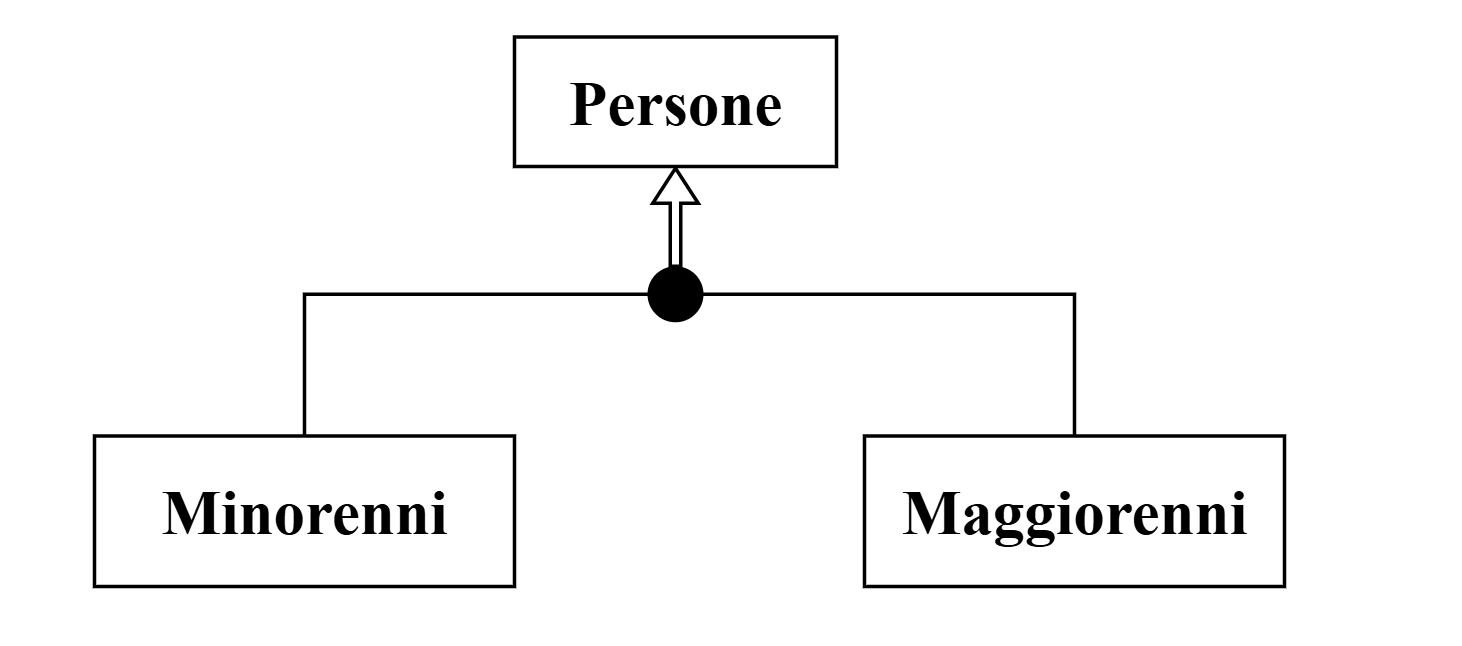
\includegraphics[width=1\textwidth, valign=t]{Diagramma disgiunzione copertura.png}
\end{minipage}\hfill
\begin{minipage}[c]{0.50\textwidth}
In questo esempio, Minorenni e Maggiorenni sono due sottoclassi esclusive e coprono anche tutte le persone, duqnue c'è sia il pallino che la doppia freccia.
\end{minipage}

\subsection{Associazioni}

\begin{Definizione}[Associazioni]
\label{def-associazioni}
Un'\textbf{associazione} è un \textbf{fatto che correla due o più entità}, creando un legame tra loro. \\
Un'associazione \textbf{R(X, Y)} fra due collezioni di entità \textbf{X} e \textbf{Y} è un \textbf{insieme di instanze di associazione} tra gli elementi di X e di Y. Il prodotto cartesiano X $\times$ Y è detto \textbf{dominio dell'associazione}. Le associazioni possono avere poi anche delle proprie \textbf{proprietà}, e possono essere anche \textbf{ricorsive} (o riflessive). \\
\NB Il concetto di associazione riprende in modo chiaro il concetto di \textbf{relazione matematica}.
\end{Definizione}

Prendiamo per esempio due insiemi di entità: l'insieme Autori = \{"Pirandello", "Leopardi"\} e l'insieme Testi = \{"Uno, Nessuno, Centomila", "La Ginestra"\}. Un'istanza di associazione sarebbe ad esempio la coppia ("Pirandello", "Uno, Nessuno, Centomila"), mentre il dominio dell'associazione sarebbe l'insieme Autori $\times$ Testi = \{("Pirandello", "Uno, Nessuno, Centomila"), ("Pirandello", "La Ginestra"),("Leopardi", "Uno, Nessuno, Centomila"), ("Leopardi", "La Ginestra")\}.

\begin{Proprieta}[Vincolo di molteplicità]
\label{prop-vincolo-molteplicita}
Un'associazione R(X,Y) è \textbf{univoca rispetto a X} se per ogni elemento x di X esiste al più un elemento y di Y associato a x. Se questo vincolo non è rispettato, allora l'associazione è \textbf{multivalore rispetto a X}.
\end{Proprieta}

\begin{itemize}
    \item R(X,Y) è \textbf{(1:N)} se è \textit{multivalore su X} e \textit{univoca su Y}. Infatti, preso un elemento y di Y, esiste solo una corrispondenza in X, mentre preso un elemento x in X esistono più corrispondenze in Y.
    \item R(X,Y) è \textbf{(N:1)} se è \textit{univoca su X} e \textit{multivalore su Y}.
    \item R(X,Y) è \textbf{(N:M)} se è \textit{multivalore su X} e \textit{multivalore su Y}.
    \item R(X,Y) è \textbf{(1:1)} se è \textit{univoca su X} e \textit{univoca su Y}.
\end{itemize}

Ad esempio, l'associazione Frequenta(Studenti, Corsi) ha \textbf{cardinalità} (N:M). Infatti, uno studente può frequentare più corsi e un corso può essere frequentato da più studenti, mentre l'associazione NatoA(Persone,Città) ha cardinalità (N:1), dato che una persona può nascere in una sola città, ma in una citta possono nascere più persone.

\begin{Proprieta}[Vincolo di totalità]
\label{prop-vincolo-totalita}
Un'associazione R(X,Y) è \textbf{totale su X} se per ogni elemento x di X esiste almeno un elemento y di Y associato a x. Se questo vincolo non è rispettato, allora l'associazione è \textbf{parziale su X}.
\end{Proprieta}

Ad esempio, l'associazione Frequenta(Studenti, Corsi) è totale su Corsi, dato che non può esistere un corso non frequentato da nessuno (verrebbe cancellato), ed è totale anche su Studenti (non esiste studente che non partecipi a nessun corso: in tal caso non sarebbe uno studente). Mentre l'associazione NatoA(Persone, Città) è totale su Persone, dato che ogni persona è nata per forza in una città, ma parziale su Città, dato che può esistere una città dove non è nato nessuno.



\end{document}